\section{Experimentación y/o validación}

En base a los casos de uso implementados analizamos cada ecosistema en las siguientes categorías: costos, experiencia de desarrollo, viabilidad y performance, con el objetivo de compararlas y ver las ventajas y desventajas de cada uno.

\subsection{Costos}
¿Cuánto nos cuesta desplegar y mantener un servicio en cada ecosistema?

\subsubsection{IPFS}

\subsubsection{Blockchain}

\paragraph{Swarm}
Al deployar el sitio web es necesario contar con \textit{postage stamps} que son la manera de pagar por el uso del almacenamiento en Swarm. Cada actualización que se realice al sitio requiere de \textit{postage stamps} y, además, estos tienen fecha de vencimiento por lo que es necesario volver a pagar frecuentemente. Hay que tener en cuenta que dichos \textit{postage stamps} se pagan en la criptomoneda BZZ que fluctúa de valor con respecto al dólar estadounidense. La obtención del sitio web no requiere de costo alguno, por lo que desde el punto de vista de un usuario lector de la aplicación no sería necesario pagar.

<TODO: medir cuánto es el costo aproximado en USD o BZZ>

\paragraph{Ethereum}
Se utiliza la moneda ETH para pagar por el despliegue de cada transacción, esto incluye tanto el despliegue de cada \textit{smart contract} como también la edición de un artículo (en el caso del repositorio de conocimiento). Por lo tanto, el usuario final de la aplicación termina pagando por creación y edición de cada artículo en el repositorio de conocimiento, y por cada mensaje enviado en el mensajero en tiempo real. Por otro lado, para las operaciones de lectura no se tiene que pagar nada.

\begin{figure}[H]
    \centering
    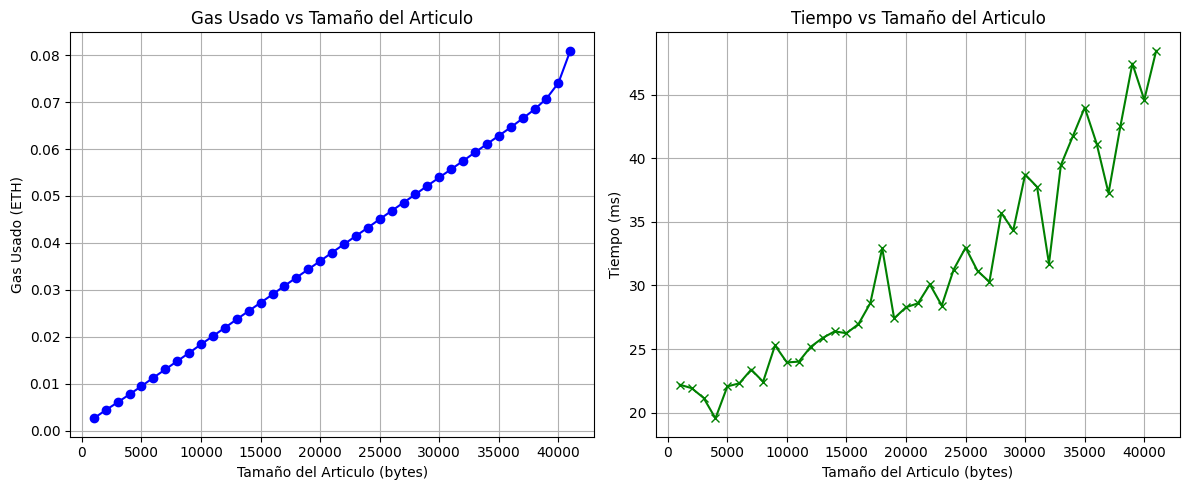
\includegraphics[width=1\linewidth]{img/aw-eth-bytes-articulo-incremental.png}
    \caption{Tiempo y gas usado al crear artículos con tamaño de bytes creciente}
    \label{fig:aw-eth-bytes-articulo-incremental.png}
\end{figure}

\subsection{Experiencia de desarrollo} % Developer Experience

¿Qué tan fácil es desplegar en cada ecosistema?

\subsubsection{IPFS}

\subsubsection{Blockchain}

\paragraph{Swarm}
En Swarm existe la herramienta de terminal \href{https://github.com/ethersphere/swarm-cli}{swarm-cli} con la cual se puede interactuar con un nodo de Swarm. También el equipo de Swarm provee una Github Action que permite la posibilidad de automatizar el despliegue generando un pipeline que utilice dicha herramienta.

En cuanto a un ambiente de pruebas o \textit{staging}, si bien no existe un \textit{gateway} público que interactúe con la \textit{testnet}, es posible levantar uno propio que sí lo haga apuntando a la \textit{testnet} de Sepolia usando la herramienta \href{https://github.com/ethersphere/gateway-proxy}{gateway-proxy}.

\paragraph{Ethereum}
Con la librería web3.js se puede interactuar con un nodo de Ethereum y realizar un despliegue de la aplicación. Además, con las herramientas de Hardhat se puede levantar una red de prueba que facilita el desarrollo local.

\subsection{Viabilidad} 

¿Que tan viable es crear una aplicación comunitaria para cada uno de estos ecosistemas?

\subsubsection{IPFS}

\subsubsection{Blockchain}

\paragraph{Swarm}
Resulta más conveniente para sitios web o recursos estáticos, al igual que IPFS. Por otro lado, al ser una tecnología de almacenamiento no es posible la ejecución de código. 

A diferencia de IPFS, Swarm cuenta con incentivos incluidos (por medio de la moneda BZZ), esto significa que para deployar contenido en la red es necesario pagar. Al hacerlo te asegura que el mismo va a estar disponible durante el tiempo equivalente al costo pagado, es decir, que no es necesario pinear los archivos puesto que se encuentran en la red con un TTL.

\paragraph{Ethereum}
Su punto fuerte es la ejecución de código, por lo cual es útil para funcionar como backend de aplicaciones web. Como hemos visto, por el costo de almacenamiento de los smart contracts, no es recomendable para recursos como imágenes, videos o incluso strings de texto muy largos como lo realizado en el repositorio de conocimiento. 

Los eventos pueden resultar útil para la interacción en tiempo real requerida en el mensajero, pero lo positivo de esto queda opacado por el hecho de necesitar pagar por cada interacción, en el caso del mensajero por cada mensaje enviado. Esto se puede volver costoso rápidamente, además de tedioso al momento de utilizar la aplicación. Se pueden explorar alternativas para reducir esta fricción, como por ejemplo, que el contrato tenga un balance de tokens para ser gastados, lo cual haría que el usuario no tenga que confirmar cada transacción de mensaje enviado si no que directamente el contrato lo extrae de su balance; entre otras posibilidades.

\subsection{Performance}

\subsubsection{IPFS}

La performance en IPFS depende de algunas variables que están fuera de nuestro alcance. Entre ellas se encuentran:
 - Uso de cache por parte de nodos de IPFS o gateways cuando se recupera un archivo.
 - Cercanía al nodo correspondiente a la hora de publicar un CID en la Distributed Hash Table.
 - Configuración y capacidades del nodo que tiene el contenido que se requiere.
 - Cantidad de nodos alojando el contenido que se requiere.

 Pese a esto, se puede minimizar el efecto de estas variables en la medida final sin distorsionar las métricas obtenidas. Más adelante se verán las maneras en las que se puede lidiar con estas variables.

\paragraph{Sitio Web Informativo}
La métrica que se decidió medir es la del \textbf{tiempo que tarda un nodo en desplegar un sitio web o contenido}. Para ello, se creó un clúster con un único nodo y un repositorio Git con contenido de distinta forma.

\subparagraph{Obtención de las métricas} En este caso, el proceso de despliegue se contiene dentro del contenedor \texttt{watcher}. Para medir el tiempo real que transcurre en cada paso del despliegue, se utilizó el comando de GNU \texttt{time} para cada paso, y el resultado es sumado para obtener el tiempo total que tardó desplegar el contenido.

\subparagraph{Archivos de prueba utilizados} Las métricas obtenidas se lograron ajustando dos variables: el tamaño total del contenido, y la cantidad de archivos del mismo. Los archivos en sí fueron generados repitiendo un \texttt{UUID} hasta alcanzar el número de bytes deseados. Se utilizó este tipo de identificador para asegurar de que ningún archivo permanezca en alguna caché, y a su vez no se repitan los CID entre archivos de la misma prueba.

%TODO: Agregar métricas de IPFS y una conclusión al respecto.

\paragraph{Astrawiki}

Las métricas tanto de Astrawiki como Astrachat se ven muy relacionadas, debido a que el grueso del trabajo relacionado a IPFS se realiza con su biblioteca en común, AstraDB. Por ejemplo, el tiempo que tarda un nodo en obtener una nueva versión de un articulo es el similar al que tarda un nodo en recibir un mensaje. Por ello, se prefirió complementar las métricas obtenidas para acentuar el uso específico de AstraDB de cada caso de uso, y evitar métricas repetidas. 

\paragraph{Astrachat}

\subsubsection{Blockchain}

\paragraph{Astrachat-eth}

Las siguientes métricas corresponden a Astrachat. Se obtuvieron levantando una instancia local de Hardhat \cite{hardhat} y ejecutando 1000 muestras. A partir de los datos obtenidos se consiguieron el máximo (\textbf{Max}), mínimo (\textbf{Min}), media (\textbf{Mean}), desvío estándar (\textbf{Std}) y la mediana (\textbf{Median}).

\subparagraph{Tiempo en enviar un mensaje}

La primer métrica tomada corresponde al tiempo que tarda en enviarse un mensaje corto (\textit{Lorem ipsum}).

\setlength\tabcolsep{1pt}
\begin{table}[!htbp]
    \centering
    \begin{tabular}{|m{5em}|m{5em}|}
    \hline
    \textbf{Max} & 11.69 ms \\
    \hline
    \textbf{Mean} & 6.15 ms \\
    \hline
    \textbf{Min} & 5.05 ms \\
    \hline
    \textbf{Std} & 0.80 ms \\
    \hline
    \textbf{Median} & 6.04 ms \\
    \hline
    \end{tabular}
    \caption{Tiempo en enviar un mensaje}
\end{table}

\subparagraph{Gas usado para enviar un mensaje}

La siguiente tabla muestra el valor (en ETH y USD) de enviar el mismo mensaje corto. El precio tomado para la conversión de ETH a dólar es el de la fecha del 1 de junio de 2025 a las 22:05 hs de \$2536.14 de la página \href{https://coinmarketcap.com/currencies/ethereum/}{Coinmarketcap}.

\setlength\tabcolsep{1pt}
\begin{table}[!htbp]
    \centering
    \begin{tabular}{|m{5em}|m{6em}|m{3em}|}
    \hline
    & \textbf{ETH} & \textbf{USD} \\
    \hline
    \textbf{Max} & 0.00049158 & 1.25 \\
    \hline
    \textbf{Mean} & 0.00034321 & 0.87 \\
    \hline
    \textbf{Min} & 0.00034239 & 0.87 \\
    \hline
    \textbf{Std} & 0.00000715 & 0.02 \\
    \hline
    \textbf{Median} & 0.00034239 & 0.87 \\
    \hline
    \end{tabular}
    \caption{Gas usado para enviar un mensaje}
\end{table}

\subparagraph{Tiempo en obtener mensajes}

Para esta métrica se tomó el tiempo en obtener todos los mensajes para un chat el cual iba teniendo cada vez más mensajes (desde 0 hasta 1000 mensajes). El gráfico muestra como el tiempo (en milisegundos) se va incrementando a medida que hay más mensajes en el chat.

\begin{figure}[h!]
    \centering
    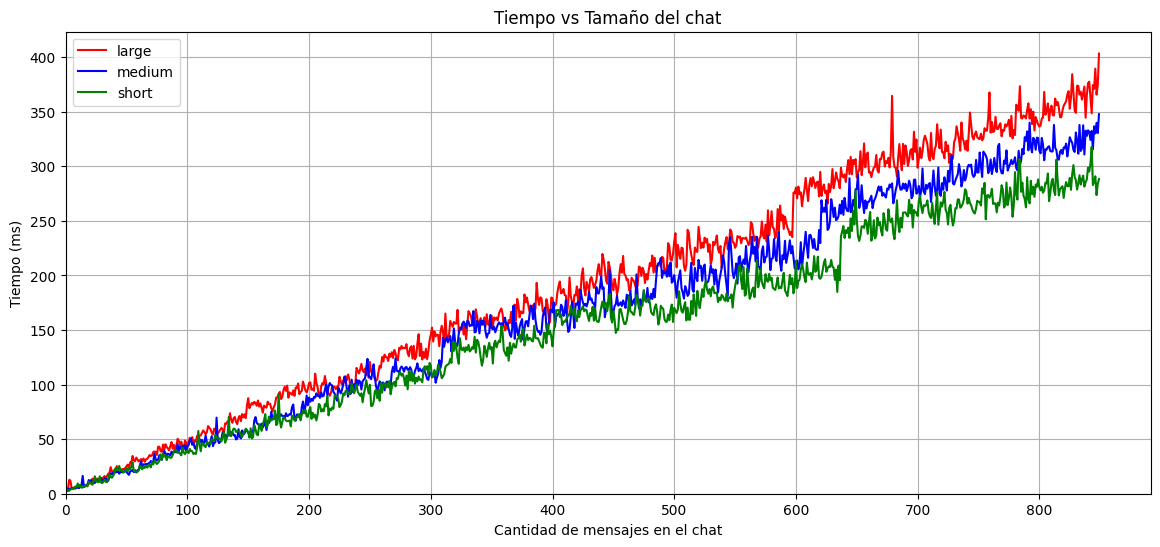
\includegraphics[width=1\linewidth]{img/blockchain-get-message-graphic.png}
    \caption{Tiempo para obtener mensajes de un chat según el tamaño del chat}
    \label{fig:blockchain-get-message-graphic.png}
\end{figure}

\subparagraph{Tiempo entre enviar y recibir un mensaje (mismo usuario)}

En esta métrica se midió el tiempo que tarda en un mensaje desde que es enviado a ser recibido por el canal de escucha de nuevos mensajes para un mismo usuario.

\setlength\tabcolsep{1pt}
\begin{table}[!htbp]
    \centering
    \begin{tabular}{|m{5em}|m{5em}|}
    \hline
    \textbf{Max} & 9.70 ms \\
    \hline
    \textbf{Mean} & 5.51 ms \\
    \hline
    \textbf{Min} & 4.37 ms \\
    \hline
    \textbf{Std} & 1.14 ms \\
    \hline
    \textbf{Median} & 4.79 ms \\
    \hline
    \end{tabular}
    \caption{Tiempo en enviar y recibir un mensaje (mismo usuario)}
\end{table}

\subparagraph{Tiempo entre enviar y recibir un mensaje (distintos usuarios)}

Esta métrica calcula el tiempo que tarda un segundo usuario en recibir un mensaje enviado por un primer usuario.

\setlength\tabcolsep{1pt}
\begin{table}[!htbp]
    \centering
    \begin{tabular}{|m{5em}|m{5em}|}
    \hline
    \textbf{Max} & 13.46 ms \\
    \hline
    \textbf{Mean} & 5.75 ms \\
    \hline
    \textbf{Min} & 4.68 ms \\
    \hline
    \textbf{Std} & 0.93 ms \\
    \hline
    \textbf{Median} & 5.27 ms \\
    \hline
    \end{tabular}
    \caption{Tiempo en enviar y recibir un mensaje (distintos usuarios)}
\end{table}

\subsection{Resumen}

\setlength\tabcolsep{1pt}
\begin{table}[H]
    \centering
    \begin{tabular}{||m{7em}|m{14em}|m{14em}||}
    \hline
     & \textbf{IPFS} & \textbf{Blockchain} \\
    \hline\hline
    \textbf{Costos} & Bajos o nulos & Escala con el uso de la aplicación \\
    \hline
    \textbf{Desarrollo} &  & Existen herramientas que facilitan el desarrollo y el despliegue \\
    \hline
    \textbf{Viabilidad} & & Sitios estáticos y aplicaciones CRUD \\
    \hline
    \textbf{Performance} & & \\
    \hline
    \end{tabular}
    \caption{Comparación entre los ecosistemas de IPFS y Blockchain}
\end{table}

% TODO: Poner la tabla, hay una en el notion 